\section{Gestione amministrativa della revisione}
\subsection{Comunicazione e risoluzione di anomalie}
Un'anomalia consiste in un comportamento non coerente con le aspettative. Un esempio di anomalie che possono essere riscontrate sono:
\begin{itemize}
	\item Violazione delle norme tipografiche da parte di un documento;
	\item Incongruenza del prodotto con funzionalità indicate nell'analisi dei requisiti.
\end{itemize}
Lo strumento scelto per la gestione delle anomalie è la sezione ``Issue'' messa a disposizione da Github$_G$. Coerentemente con l'organizzazione generale delle strategie di verifica, nuove anomalie potranno essere scoperte in due modi:

\begin{itemize}
	\item In ogni fase di verifica, il \ruoloVerificatore\ avrà il compito di cercare eventuali anomalie;
	\item Grazie all'approccio ``Broken Window Theory'' (vedi sezione 2.1), chiunque in qualunque momento è incentivato alla ricerca di possibili anomalie.
\end{itemize}
Nel caso in cui un \ruoloVerificatore\ o un membro del gruppo individui un anomalia dovrà segnalarlo aprendo un ticket$_G$ (vedi documento allegato \textit{NormeDiProgetto\_v3.0.pdf} sezione 5.2). Un \ruoloVerificatore\ ha il compito di controllare le pull request quindi nel caso trovasse un anomalia deve impedire la pull request con le modalità descritte nella sezione 5.4 delle \textit{NormeDiProgetto\_v3.0.pdf}.

\subsection{Trattamento delle discrepanze}
Una discrepanza è un discostamento dai requisiti attesi del capitolato o una violazione delle Norme di Progetto. Il trattamento delle discrepanze avviene come la gestione delle anomalie. Quando un membro del gruppo o il \ruoloVerificatore\ ne individuasse una segnalerà il problema aprendo un ticket$_G$ oppure un \ruoloVerificatore\ può bloccare la pull specificando il motivo al richiedente come per il trattamento delle anomalie.
\newpage\right 
\subsection{Procedure di controllo di qualità di processo}

Come accennato nella sezione 3.2.1, l'organizzazione dei processi fa riferimento al ciclo di Deming, che ha come scopo il miglioramento continuo, secondo il principio del PDCA. Questo garantisce un miglioramento continuo di tutti i processi e delle attività di verifica che si realizza con comunicazioni attive delle componenti del gruppo e con la connessione delle fasi di analisi, progettazione, verifica e collaudo. La qualità dei processi viene monitorata anche grazie alla qualità di prodotto perché un prodotto di bassa qualità può indicare che uno o più processi vadano migliorati. Per questo motivo si presta attenzione a monitorare i singoli processi ed è necessario quindi che i processi vengano pianificati nel dettaglio, le risorse vengano ripartite nella pianificazione in modo chiaro e ci sia un adeguato controllo sui processi. Tale metodo è suddiviso in quattro fasi:

\begin{enumerate}
	\item \textbf{Plan - Pianificare}:
		\begin{itemize}
			\item[(a)] Definire il problema/impostare il progetto;
			\item[(b)] Documentare la situazione di partenza;
			\item[(c)] Analizzare il problema;
			\item[(d)] Pianificare le azioni da realizzare.
		\end{itemize}

	\item \textbf{Do - Realizzare}:
		\begin{itemize}
			\item[(a)] Addestrare le persone incaricate della realizzazione;
			\item[(b)] Realizzare le azioni che sono state pianificate.
		\end{itemize}
	
	\item \textbf{Check -Verificare}:
		\begin{itemize}
			\item[(a)] Verificare i risultati e confrontarli con gli obiettivi;
			\item[(b)] Se si `e raggiunto l'obiettivo: passare alla lettera a della fase Act;
			\item[(c)] Se non si è raggiunto l'obiettivo: passare alla lettera b della fase Act.
		\end{itemize}
	
	\item \textbf{Act - Mantenere o Migliorare}:
		\begin{itemize}
			\item[(a)] Obiettivo raggiunto:
				\begin{itemize}
					\item[i.] Standardizzare, consolidare e addestrare gli operatori;
					\item[ii.] Procedere a un nuovo PDCA per un ulteriore miglioramento sul tema.
				\end{itemize}
			\item[(b)] Obiettivo non raggiunto:
				\begin{itemize}
					\item[i.] Ripetere il ciclo PDCA sullo stesso problema, analizzando criticamente le varie fasi del ciclo precedente per individuare le cause del non raggiungimento dell'obiettivo.
				\end{itemize}
		\end{itemize} 
\end{enumerate}  \pagebreak \\

\begin{figure}[h!]
	\centering
	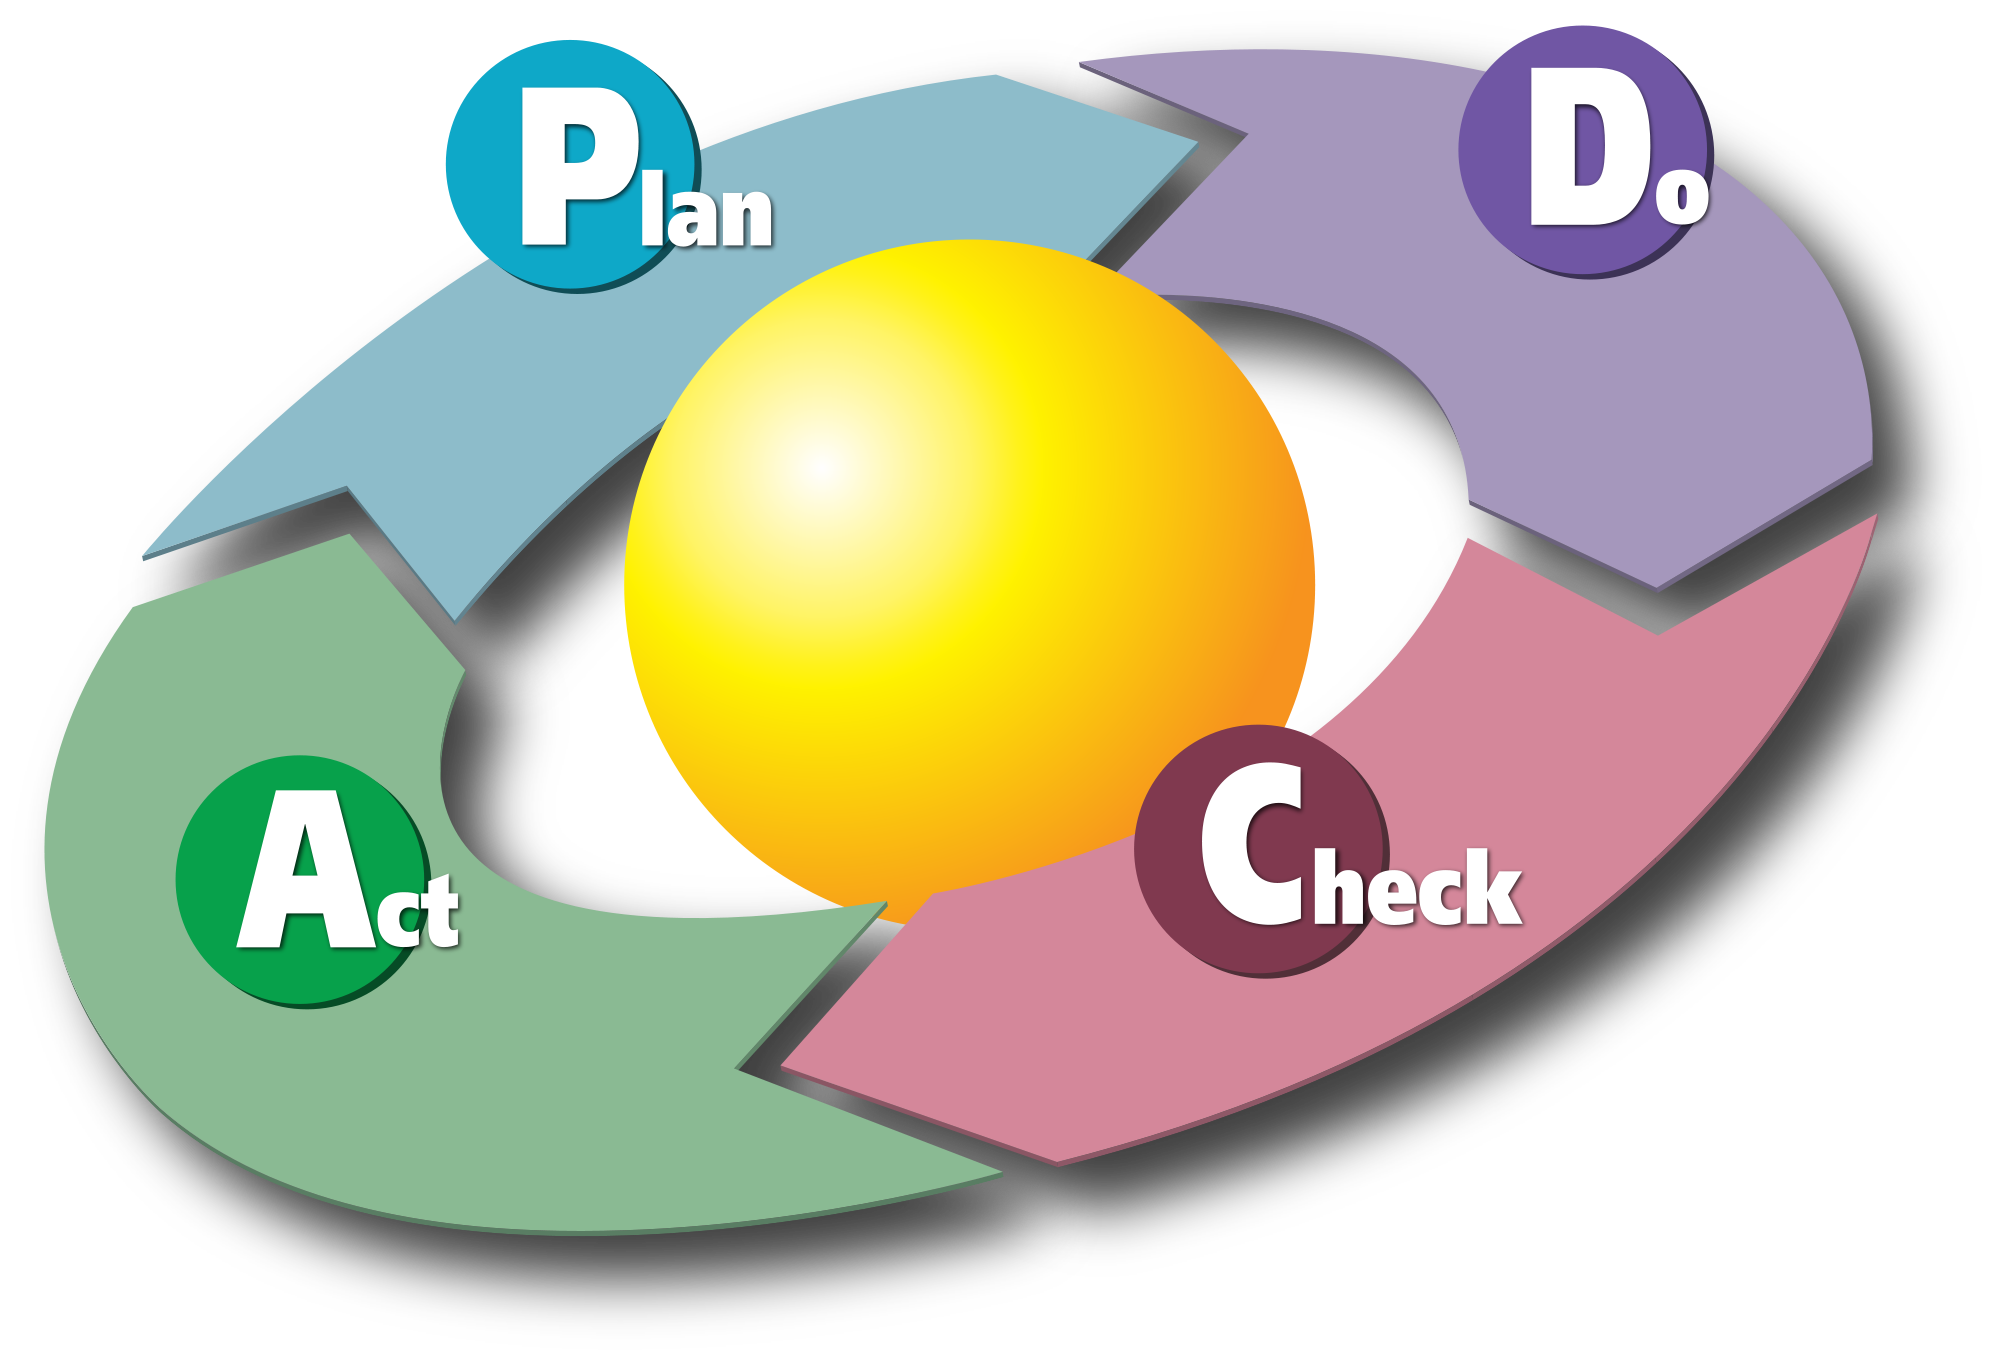
\includegraphics[scale=.2]{img/2000px-PDCA_Cycle.png}
	\caption{Modello PDCA}
	\label{fig:ModelloPDCA}
\end{figure} 

I parametri che permetteranno di valutare la qualità del processo saranno principalmente:
\begin{itemize}
	\item il tempo impiegato per essere portato a termine; 
	\item la quantità di risorse impiegate;
	\item il numero di iterazioni che è stato fatto;
	\item il numero di difetti trovati durante la fase di testing.
\end{itemize}
Tali parametri devono essere quantificati sia durante che al termine del processo, al fine di individuare eventuali problemi e capire, attraverso un'analisi condivisa dai membri del gruppo, in quali aree c'è bisogno di un miglioramento. Alla successiva istanziazione del processo, i dati raccolti la volta precedente vanno capiti e migliorati in modo da rendere più efficiente ed efficace il processo stesso. \\ \\
Il gruppo \gruppo adotta come riferimento lo standard ISO/IEC$_G$ 14598 che descrive il processo di valutazione della qualità del software, in accordo con la norma ISO/IEC 9126 descritta nel capitolo 3. Esse verranno utilizzate per valutare il software durante tutto il suo ciclo di vita. La figura seguente schematizza il processo di valutazione:

\begin{figure}[h!]
	\centering
	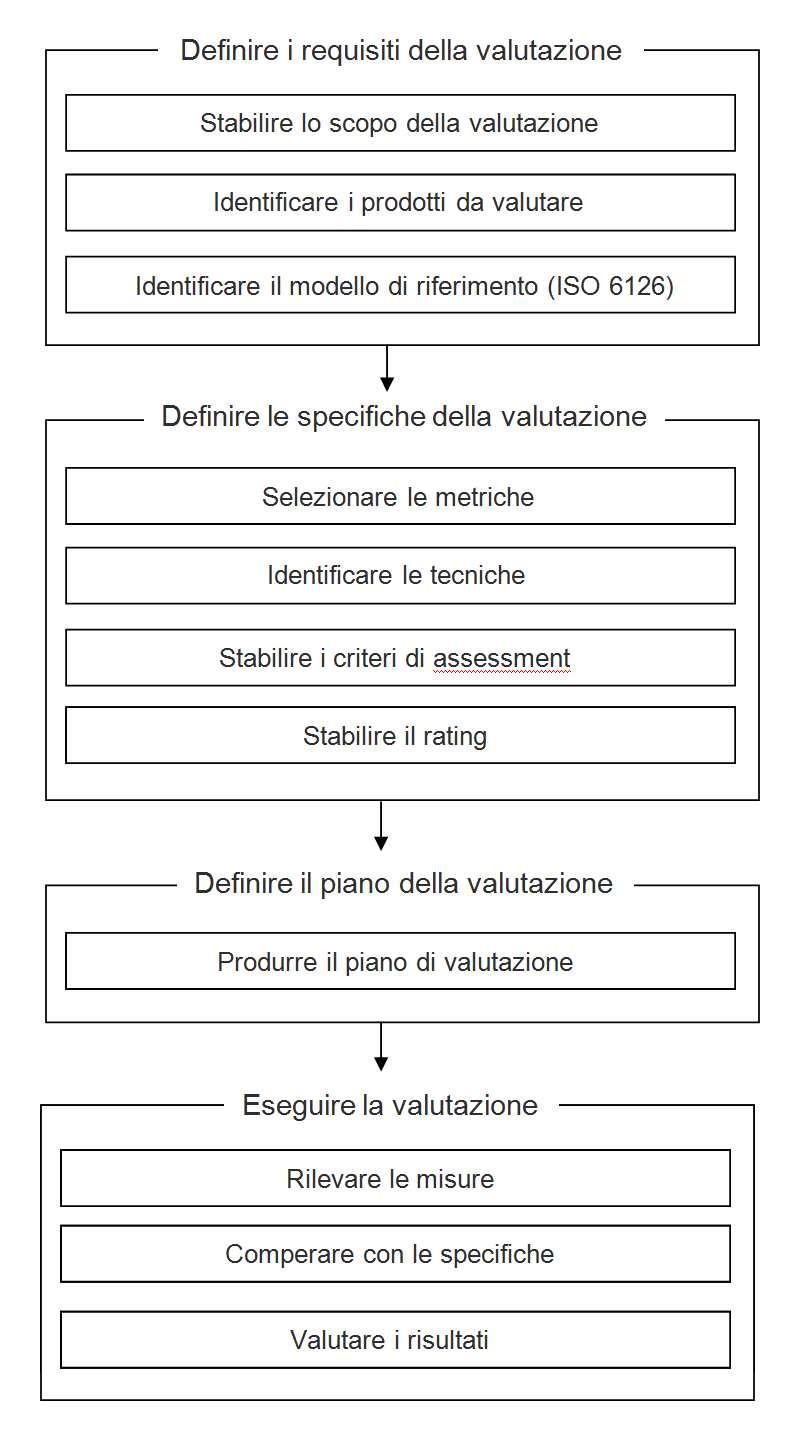
\includegraphics[scale=.6]{img/schema_VAL.png}
	\caption{Il Processo di Valutazione}
	\label{fig:Il Processo di Valutazione}
\end{figure} 

\pagebreak
